% Auriga theme
% https://github.com/anishathalye/auriga

\documentclass[14pt,aspectratio=169]{beamer}
\usepackage{pgfpages}
\usepackage{fancyvrb}
\usepackage{tikz}
\usepackage{pgfplots}
\usepackage{graphicx}

\graphicspath{ {./assets/img/} }

\ifnotes
\setbeamertemplate{note page}[plain]
\setbeameroption{show notes on second screen=right}
\fi

\usetheme{auriga}
\usecolortheme{auriga}

% define some colors for a consistent theme across slides
\definecolor{red}{RGB}{181, 23, 0}
\definecolor{blue}{RGB}{0, 118, 186}
\definecolor{gray}{RGB}{146, 146, 146}

\title{StackQL: head in the clouds, feet on the ground}

\author{\underline{Kieran Rimmer} \inst{1} \inst{1} \and Jeffrey Aven \inst{1} \inst{3}}

\institute[shortinst]{\inst{1} StackQL Studios \samelineand \inst{2} Ryuk IT \and \inst{3} Aven Solutions  }

\begin{document}

{
  % rather than use the frame options [noframenumbering,plain], we make the
  % color match, so that the indicated page numbers match PDF page numbers
  \setbeamercolor{page number in head/foot}{fg=background canvas.bg}
  \begin{frame}
    \titlepage
  \end{frame}
}

\begin{frame}{Background}

  \begin{itemize}
    \item Professional Services
    \item IAC ideation
    \item Begun with Google only
    \item CyRise Cohort 6 (2022)
      \begin{itemize}
        \item Compliance and Audit
        \item \textbf{Viz}
      \end{itemize}
  \end{itemize}

  \note{
    Here's a note for this slide.
  }

\end{frame}

\begin{frame}{Philosophy}

  \begin{itemize}
    \item Community first
      \begin{itemize}
        \item All open source
        \item Inspired by our idols
      \end{itemize}
    \item Composable tooling for all
    \item Why golang?
      \begin{itemize}
        \item Java / JVM fatigue
        \item Why \textbf{not}?
      \end{itemize}
  \end{itemize}

  \note{
    Here's a note for this slide.
  }

\end{frame}

\input{slides/bullets}
\begin{frame}{High Level Design}

  \begin{columns}
    \begin{column}{0.5\linewidth}
      \begin{itemize}
        \item Reusable Componentry
        \item Loads of Forks
        \item See \href{https://github.com/stackql/stackql/blob/main/docs/high-level-design.md} {doco}
      \end{itemize}
    \end{column}
    \begin{column}{0.5\linewidth}
      \begin{figure}
        \centering
          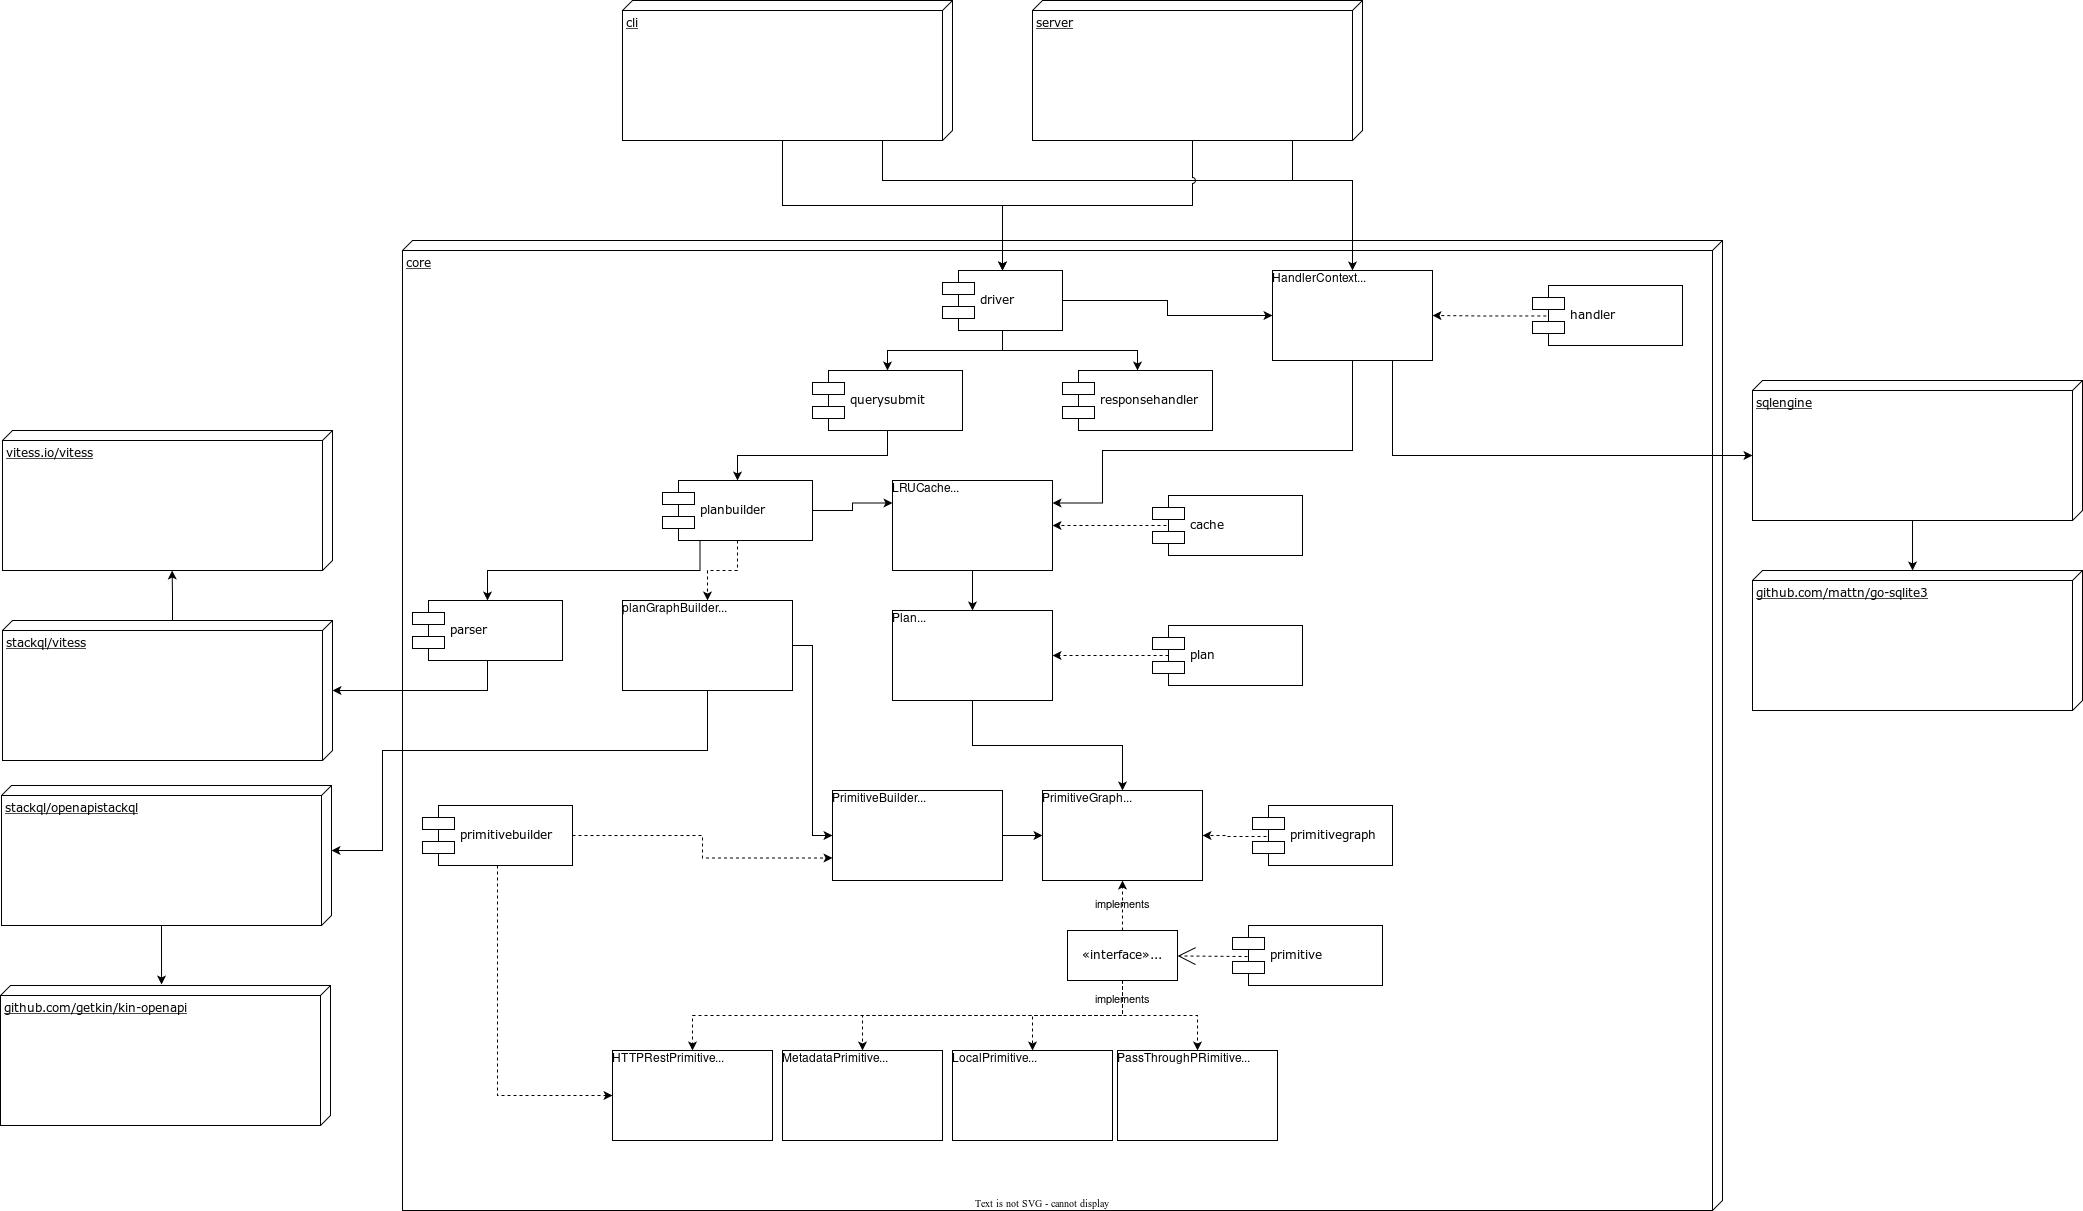
\includegraphics[width=5cm, height=4cm]{hldd}
        \caption{A figure caption}
      \end{figure}
    \end{column}
  \end{columns}

  \note{
    This slide has notes too.
  }

\end{frame}

\input{slides/figure}
\input{slides/centered}
\input{slides/monospace}
\input{slides/brackets}
\input{slides/link}

\end{document}
